% Author and sole contributor: Lazaros Varvatis.
\subsection{Pre-specified multi-seed check of Toy V2}
\label{sec:toy2robustness}
\begingroup
\emergencystretch=3em

\paragraph{Protocol, amendment and chronology.}
The original design was committed as
\href{https://github.com/LAKITALKS/LEM/commit/c7d44d1dcbfc1bef889601dda69dcc95b8500cb3}{\texttt{c7d44d1}}
before any computation. Its outputs were committed as \texttt{ee90b9f}.
Amendment 1, dated 8 November 2026, was then supplied following external review
and committed as
\href{https://github.com/LAKITALKS/LEM/commit/cf66e01fb868d829948cea0bc8c7b550181f208c}{\texttt{cf66e01}}
before supplemental computation. Its purpose was to compare $H_1$ with a joint
geometric predictor, add a uniform control, and explicitly test invariance to
temporal shuffling. The original results had already been computed, inspected by
the executing assistant and reported in the chat before the amendment arrived.
Thus the amended analysis is not presented as preceding all access to the original
results. Both frozen versions are reported; original output hashes remain unchanged.
The exact specifications and seed assignments are in
\href{https://github.com/LAKITALKS/LEM/blob/v2.3-toy-v2-robustness/experiments/toy_v2_robustness/PROTOCOL.md}{\texttt{PROTOCOL.md}}.

\paragraph{Generators, controls and measurement window.}
We retain the original sink and Van der Pol generators, numerical integration,
initial conditions, $\mu=1.5$, $\lambda=0.5$, $T=40$ and $\Delta t=0.1$.
The window $W$ consists of all 401 points entering persistence, including
transients; the original has no burn-in removal or subsampling. Numerical helper
functions were copied verbatim, with only dedentation, from
\texttt{experiments/lem\_simulations.py} at source commit \texttt{e2c0487}
(lines 591--615), and checked against that source.

The amended name \textbf{GAUSS} denotes the original \textbf{DISK}: a stationary
2-D Gaussian OU process discretized as AR(1). Its common lag-1 coefficient is
estimated by pooling the centered CYCLE coordinates on $W$. The start is drawn
from the stationary distribution. The realized sample is then centered, whitened
by its own sample covariance, colored by CYCLE's sample covariance and shifted
to CYCLE's mean. \textbf{UNIFORM} starts with independent uniform points in an
ellipse and undergoes the same exact finite-sample affine moment matching.
The sample-dependent matching step couples the final points; uniformity and
independence describe the initial draws. \textbf{LINE} is a finite sinusoid on
CYCLE's first principal axis, with the dominant nonzero FFT frequency and exact
sample mean and total-variance matching. Its amplitude uses the finite
sinusoid's sample variance, not $A^2/2$.

A common unnormalized Gaussian $2\times16$ projection per seed is primary;
independent projections per trajectory are secondary. Independent Gaussian
observation noise is added after projection. Original random streams and
per-seed statistics are preserved; UNIFORM uses a separate control stream and is
appended after the original classes in the embedding stream. Before observation
noise, the GAUSS/UNIFORM moment matching also matches $g_1$ and $g_2$ under a
common projection; these serve as plausibility checks, not as the main
individual geometric competitor.

\paragraph{Statistics, frozen predictors and uncertainty.}
The individual statistics are maximum finite Vietoris--Rips $H_1$ lifetime;
$g_1$, the radius of gyration on all $W$; $g_2$, the largest divided by the
second-largest PCA covariance eigenvalue; and $g_3$, the coefficient of variation
of centroid distances in the first two principal components. We additionally
report $g_{1,\mathrm{half}}$ on the second half for comparability; it does not enter
categorization. For each statistic/comparison/noise/projection, sign and threshold
are selected on calibration seeds by Youden's criterion and frozen.

The joint geometric predictor $G$ is logistic regression on standardized
$(g_1,g_2,g_3)$; $G+H_1$ additionally includes $H_1$. Both use L2 regularization
with $C=1.0$ fixed. Scalers and models are fitted exclusively to calibration
seeds, with no subsequent tuning. The control is the positive class. For $G$
and $G+H_1$, accuracy uses the fixed probability cutoff $0.5$; $H_1$ accuracy uses
its original frozen threshold. At noise $0.05$, seeds 0--99 calibrate and
100--199 evaluate, with all classes sharing each seed. At each other noise
level ($0.01,0.025,0.1,0.2,0.5$), seeds 0--19 calibrate and 20--39 evaluate.
Levels and projection modes are never pooled. Percentile 95\% bootstrap
intervals use 1000 resamples of whole evaluation seeds (fixed seed 2300), keeping
all classes and predictions of each seed together. Models, signs and thresholds
are not refitted in resamples; $\Delta$AUC uses paired differences from those
same resamples.

\begin{table}[htbp]
\centering\small\setlength{\tabcolsep}{4pt}
\caption{Amendment 1 main evaluation: CYCLE versus each control, noise $0.05$,
common projection, 100 evaluation seeds per class. Entries show AUC and paired
95\% bootstrap interval; $\Delta$AUC is AUC$(G+H_1)-$AUC$(G)$.}
\label{tab:toy2amendedauc}
% Generated only from the committed numerical summaries.
\begin{tabular}{lcccc}
\toprule
Control & $H_1$ & $G$ & $G+H_1$ & $\Delta$AUC \\
\midrule
GAUSS & \shortstack{0.9942\\(0.9842, 1.0000)} & \shortstack{0.8276\\(0.7547, 0.8859)} & \shortstack{0.9933\\(0.9793, 1.0000)} & \shortstack{0.1657\\(0.1087, 0.2347)} \\[3pt]
UNIFORM & \shortstack{1.0000\\(1.0000, 1.0000)} & \shortstack{0.5745\\(0.4824, 0.6677)} & \shortstack{1.0000\\(1.0000, 1.0000)} & \shortstack{0.4255\\(0.3323, 0.5176)} \\[3pt]
LINE & \shortstack{1.0000\\(1.0000, 1.0000)} & \shortstack{1.0000\\(1.0000, 1.0000)} & \shortstack{1.0000\\(1.0000, 1.0000)} & \shortstack{0.0000\\(0.0000, 0.0000)} \\[3pt]
\bottomrule
\end{tabular}

\end{table}

\begin{table}[htbp]
\centering\small
\caption{Accuracy under the frozen $H_1$ threshold or fixed logistic probability
cutoff $0.5$, with 95\% bootstrap intervals, on the same amended primary evaluation.}
\label{tab:toy2amendedaccuracy}
% Generated only from the committed numerical summaries.
\begin{tabular}{lccc}
\toprule
Control & $H_1$ & $G$ & $G+H_1$ \\
\midrule
GAUSS & \shortstack{0.9850\\(0.9650, 1.0000)} & \shortstack{0.7750\\(0.7150, 0.8300)} & \shortstack{0.9900\\(0.9750, 1.0000)} \\[3pt]
UNIFORM & \shortstack{0.9950\\(0.9850, 1.0000)} & \shortstack{0.5950\\(0.5250, 0.6650)} & \shortstack{1.0000\\(1.0000, 1.0000)} \\[3pt]
LINE & \shortstack{1.0000\\(1.0000, 1.0000)} & \shortstack{1.0000\\(1.0000, 1.0000)} & \shortstack{1.0000\\(1.0000, 1.0000)} \\[3pt]
\bottomrule
\end{tabular}

\end{table}

\paragraph{Amended decision rules and result.}
Categories are determined separately for GAUSS and UNIFORM on the primary
evaluation. \textit{EINDEUTIGER VORTEIL} requires AUC$(H_1)\geq0.95$ and
AUC$(G)\leq0.65$. \textit{ZUSATZNUTZEN} requires AUC$(H_1)\geq0.95$,
AUC$(G)>0.65$, $\Delta$AUC$\geq0.05$, and a strictly positive lower
95\% bootstrap limit for $\Delta$AUC. \textit{GLEICHSTAND} applies when
AUC$(H_1)\geq0.95$ and neither preceding condition holds.
\textit{NICHT ROBUST} applies when AUC$(H_1)<0.95$: $H_1$ alone does not
recognize the constructed loop reliably, not ``not significant.'' The overall
category is the weaker of the two, ordered as these four labels above.
LINE is a plausibility probe and does not enter categorization.

The amended primary result is \textbf{ZUSATZNUTZEN} for GAUSS and
\textbf{EINDEUTIGER VORTEIL} for UNIFORM; the overall category is
\textbf{ZUSATZNUTZEN}. Against GAUSS, $H_1$ AUC is $0.9942$
$[0.9842,1.0000]$, $G$ AUC is $0.8276$ $[0.7547,0.8859]$, and $G+H_1$
AUC is $0.9933$ $[0.9793,1.0000]$; the paired increment is $0.1657$
$[0.1087,0.2347]$. Against UNIFORM the corresponding AUCs are $1.0000$,
$0.5745$ and $1.0000$, with increment $0.4255$ $[0.3323,0.5176]$.
These categories apply only to the specified toy controls and fixed predictors;
they do not establish an advantage over all geometric methods.

\begin{table}[p]
\centering\small
\caption{Amended primary evaluation: individual statistics, AUC and accuracy with
95\% bootstrap intervals. The comparison is CYCLE versus the named control;
$g_{1,\mathrm{half}}$ is supplementary and order-dependent.}
\label{tab:toy2amendedgeometry}
% Generated only from the committed numerical summaries.
\begin{tabular}{llcc}
\toprule
Comparison / control & Statistic & AUC (95\% CI) & Accuracy (95\% CI) \\
\midrule
GAUSS & $H_1$ & \shortstack{0.9942\\(0.9842, 1.0000)} & \shortstack{0.9850\\(0.9650, 1.0000)} \\[3pt]
GAUSS & $g_1$ & \shortstack{0.5000\\(0.4962, 0.5031)} & \shortstack{0.5000\\(0.5000, 0.5000)} \\[3pt]
GAUSS & $g_2$ & \shortstack{0.5003\\(0.4968, 0.5045)} & \shortstack{0.5000\\(0.5000, 0.5000)} \\[3pt]
GAUSS & $g_3$ & \shortstack{0.8321\\(0.7637, 0.8843)} & \shortstack{0.7000\\(0.6449, 0.7550)} \\[3pt]
GAUSS & $g_{1,\mathrm{half}}$ & \shortstack{0.7920\\(0.7473, 0.8369)} & \shortstack{0.7100\\(0.6599, 0.7600)} \\[3pt]
UNIFORM & $H_1$ & \shortstack{1.0000\\(1.0000, 1.0000)} & \shortstack{0.9950\\(0.9850, 1.0000)} \\[3pt]
UNIFORM & $g_1$ & \shortstack{0.5011\\(0.4983, 0.5053)} & \shortstack{0.5000\\(0.5000, 0.5000)} \\[3pt]
UNIFORM & $g_2$ & \shortstack{0.4997\\(0.4961, 0.5034)} & \shortstack{0.5000\\(0.5000, 0.5000)} \\[3pt]
UNIFORM & $g_3$ & \shortstack{0.4794\\(0.3921, 0.5634)} & \shortstack{0.6150\\(0.5650, 0.6700)} \\[3pt]
UNIFORM & $g_{1,\mathrm{half}}$ & \shortstack{0.6478\\(0.6308, 0.6755)} & \shortstack{0.6150\\(0.5750, 0.6600)} \\[3pt]
LINE & $H_1$ & \shortstack{1.0000\\(1.0000, 1.0000)} & \shortstack{1.0000\\(1.0000, 1.0000)} \\[3pt]
LINE & $g_1$ & \shortstack{0.5129\\(0.4678, 0.5590)} & \shortstack{0.5250\\(0.4800, 0.5700)} \\[3pt]
LINE & $g_2$ & \shortstack{1.0000\\(1.0000, 1.0000)} & \shortstack{0.9950\\(0.9850, 1.0000)} \\[3pt]
LINE & $g_3$ & \shortstack{0.9200\\(0.8600, 0.9700)} & \shortstack{0.9500\\(0.9150, 0.9750)} \\[3pt]
LINE & $g_{1,\mathrm{half}}$ & \shortstack{0.6381\\(0.5961, 0.6859)} & \shortstack{0.6350\\(0.5900, 0.6850)} \\[3pt]
\bottomrule
\end{tabular}

\end{table}

\begin{figure}[p]
\centering
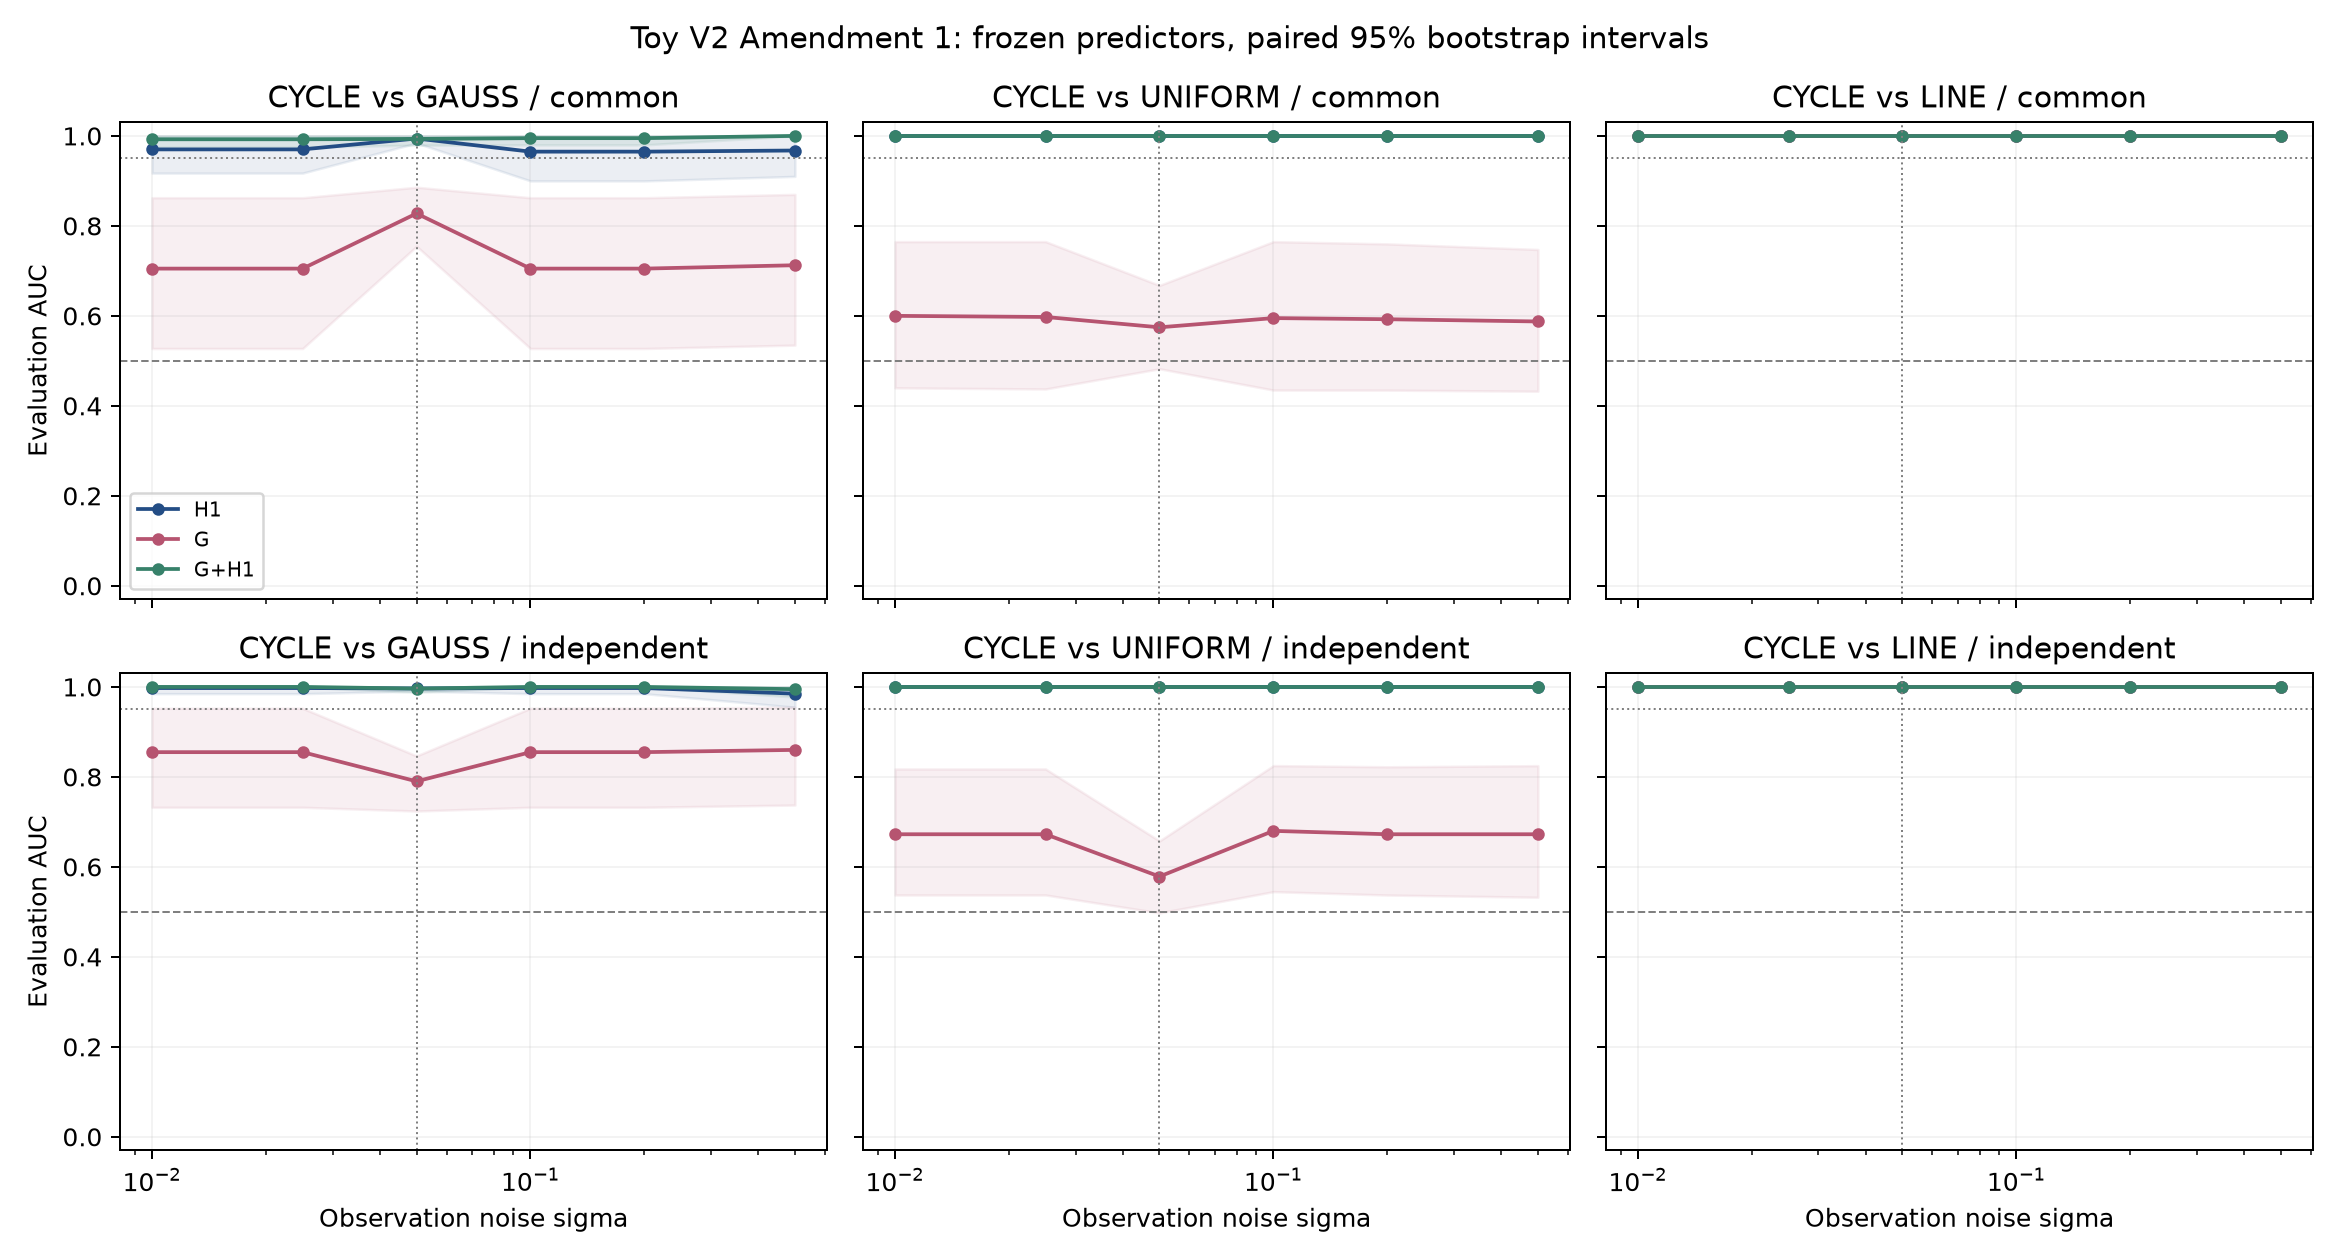
\includegraphics[width=\textwidth]{../experiments/results/toy_v2_robustness/amendment_1/toy_v2_robustness.png}
\caption{Amendment 1 noise sweep: evaluation AUCs of frozen predictors, with paired
95\% bootstrap intervals. Top: common projection; bottom: independent projections.
The primary $0.05$ point uses 100 evaluation seeds per class (100--199); all other
points use 20 (20--39). Changes across these points therefore also reflect
different evaluation seed sets. No levels are pooled.}
\label{fig:toy2amendednoise}
\end{figure}

\paragraph{Original committed analysis, retained without replacement.}
The original evaluation compared individual statistics only. R1 is
\textbf{H1 trennt Senke und Zyklus}, since AUC$(H_1,\mathrm{Va})=1.0000$.
Its R2, based solely on Vb (CYCLE versus DISK, now called GAUSS), is
\textbf{TEILWEISE}: $H_1$ AUC is $0.9942$, $g_1$ is $0.5000$,
$g_2$ is $0.5003$, and $g_3$ is $0.8321$.
The original rules classify all $g$ AUCs $\leq0.65$ as
\textit{EINDEUTIGER VORTEIL}, a best $g$ AUC strictly between $0.65$ and
$0.95$ as \textit{TEILWEISE}, any $g$ AUC $\geq0.95$ as
\textit{KEIN EINDEUTIGER VORTEIL}, conditional on $H_1$ AUC $\geq0.95$;
otherwise they assign \textit{NICHT ROBUST}.
Vc (CYCLE versus LINE) remains outside R2; its $g_2$ AUC is $1.0000$.
The different original and amended category labels reflect different specified
comparators and decision rules; one has not been substituted for the other.

\begin{table}[p]
\centering\small
\caption{Original committed primary evaluation, retained verbatim numerically:
Va: SINK versus CYCLE; Vb: CYCLE versus DISK (GAUSS); Vc: CYCLE versus LINE.
AUC and accuracy with 95\%
bootstrap intervals; signs and thresholds were frozen using calibration seeds.}
\label{tab:toy2originalmulti}
% Generated only from the committed numerical summaries.
\begin{tabular}{llcc}
\toprule
Comparison / control & Statistic & AUC (95\% CI) & Accuracy (95\% CI) \\
\midrule
Va & $H_1$ & \shortstack{1.0000\\(1.0000, 1.0000)} & \shortstack{0.9900\\(0.9750, 1.0000)} \\[3pt]
Va & $g_1$ & \shortstack{1.0000\\(1.0000, 1.0000)} & \shortstack{0.9950\\(0.9850, 1.0000)} \\[3pt]
Va & $g_2$ & \shortstack{1.0000\\(1.0000, 1.0000)} & \shortstack{0.9950\\(0.9800, 1.0000)} \\[3pt]
Va & $g_3$ & \shortstack{1.0000\\(1.0000, 1.0000)} & \shortstack{0.9950\\(0.9800, 1.0000)} \\[3pt]
Va & $g_{1,\mathrm{half}}$ & \shortstack{1.0000\\(1.0000, 1.0000)} & \shortstack{0.9950\\(0.9850, 1.0000)} \\[3pt]
Vb & $H_1$ & \shortstack{0.9942\\(0.9842, 1.0000)} & \shortstack{0.9850\\(0.9650, 1.0000)} \\[3pt]
Vb & $g_1$ & \shortstack{0.5000\\(0.4962, 0.5031)} & \shortstack{0.5000\\(0.5000, 0.5000)} \\[3pt]
Vb & $g_2$ & \shortstack{0.5003\\(0.4968, 0.5045)} & \shortstack{0.5000\\(0.5000, 0.5000)} \\[3pt]
Vb & $g_3$ & \shortstack{0.8321\\(0.7637, 0.8843)} & \shortstack{0.7000\\(0.6449, 0.7550)} \\[3pt]
Vb & $g_{1,\mathrm{half}}$ & \shortstack{0.7920\\(0.7473, 0.8369)} & \shortstack{0.7100\\(0.6599, 0.7600)} \\[3pt]
Vc & $H_1$ & \shortstack{1.0000\\(1.0000, 1.0000)} & \shortstack{1.0000\\(1.0000, 1.0000)} \\[3pt]
Vc & $g_1$ & \shortstack{0.5129\\(0.4678, 0.5590)} & \shortstack{0.5250\\(0.4800, 0.5700)} \\[3pt]
Vc & $g_2$ & \shortstack{1.0000\\(1.0000, 1.0000)} & \shortstack{0.9950\\(0.9850, 1.0000)} \\[3pt]
Vc & $g_3$ & \shortstack{0.9200\\(0.8600, 0.9700)} & \shortstack{0.9500\\(0.9150, 0.9750)} \\[3pt]
Vc & $g_{1,\mathrm{half}}$ & \shortstack{0.6381\\(0.5961, 0.6859)} & \shortstack{0.6350\\(0.5900, 0.6850)} \\[3pt]
\bottomrule
\end{tabular}

\end{table}

\begin{figure}[p]
\centering
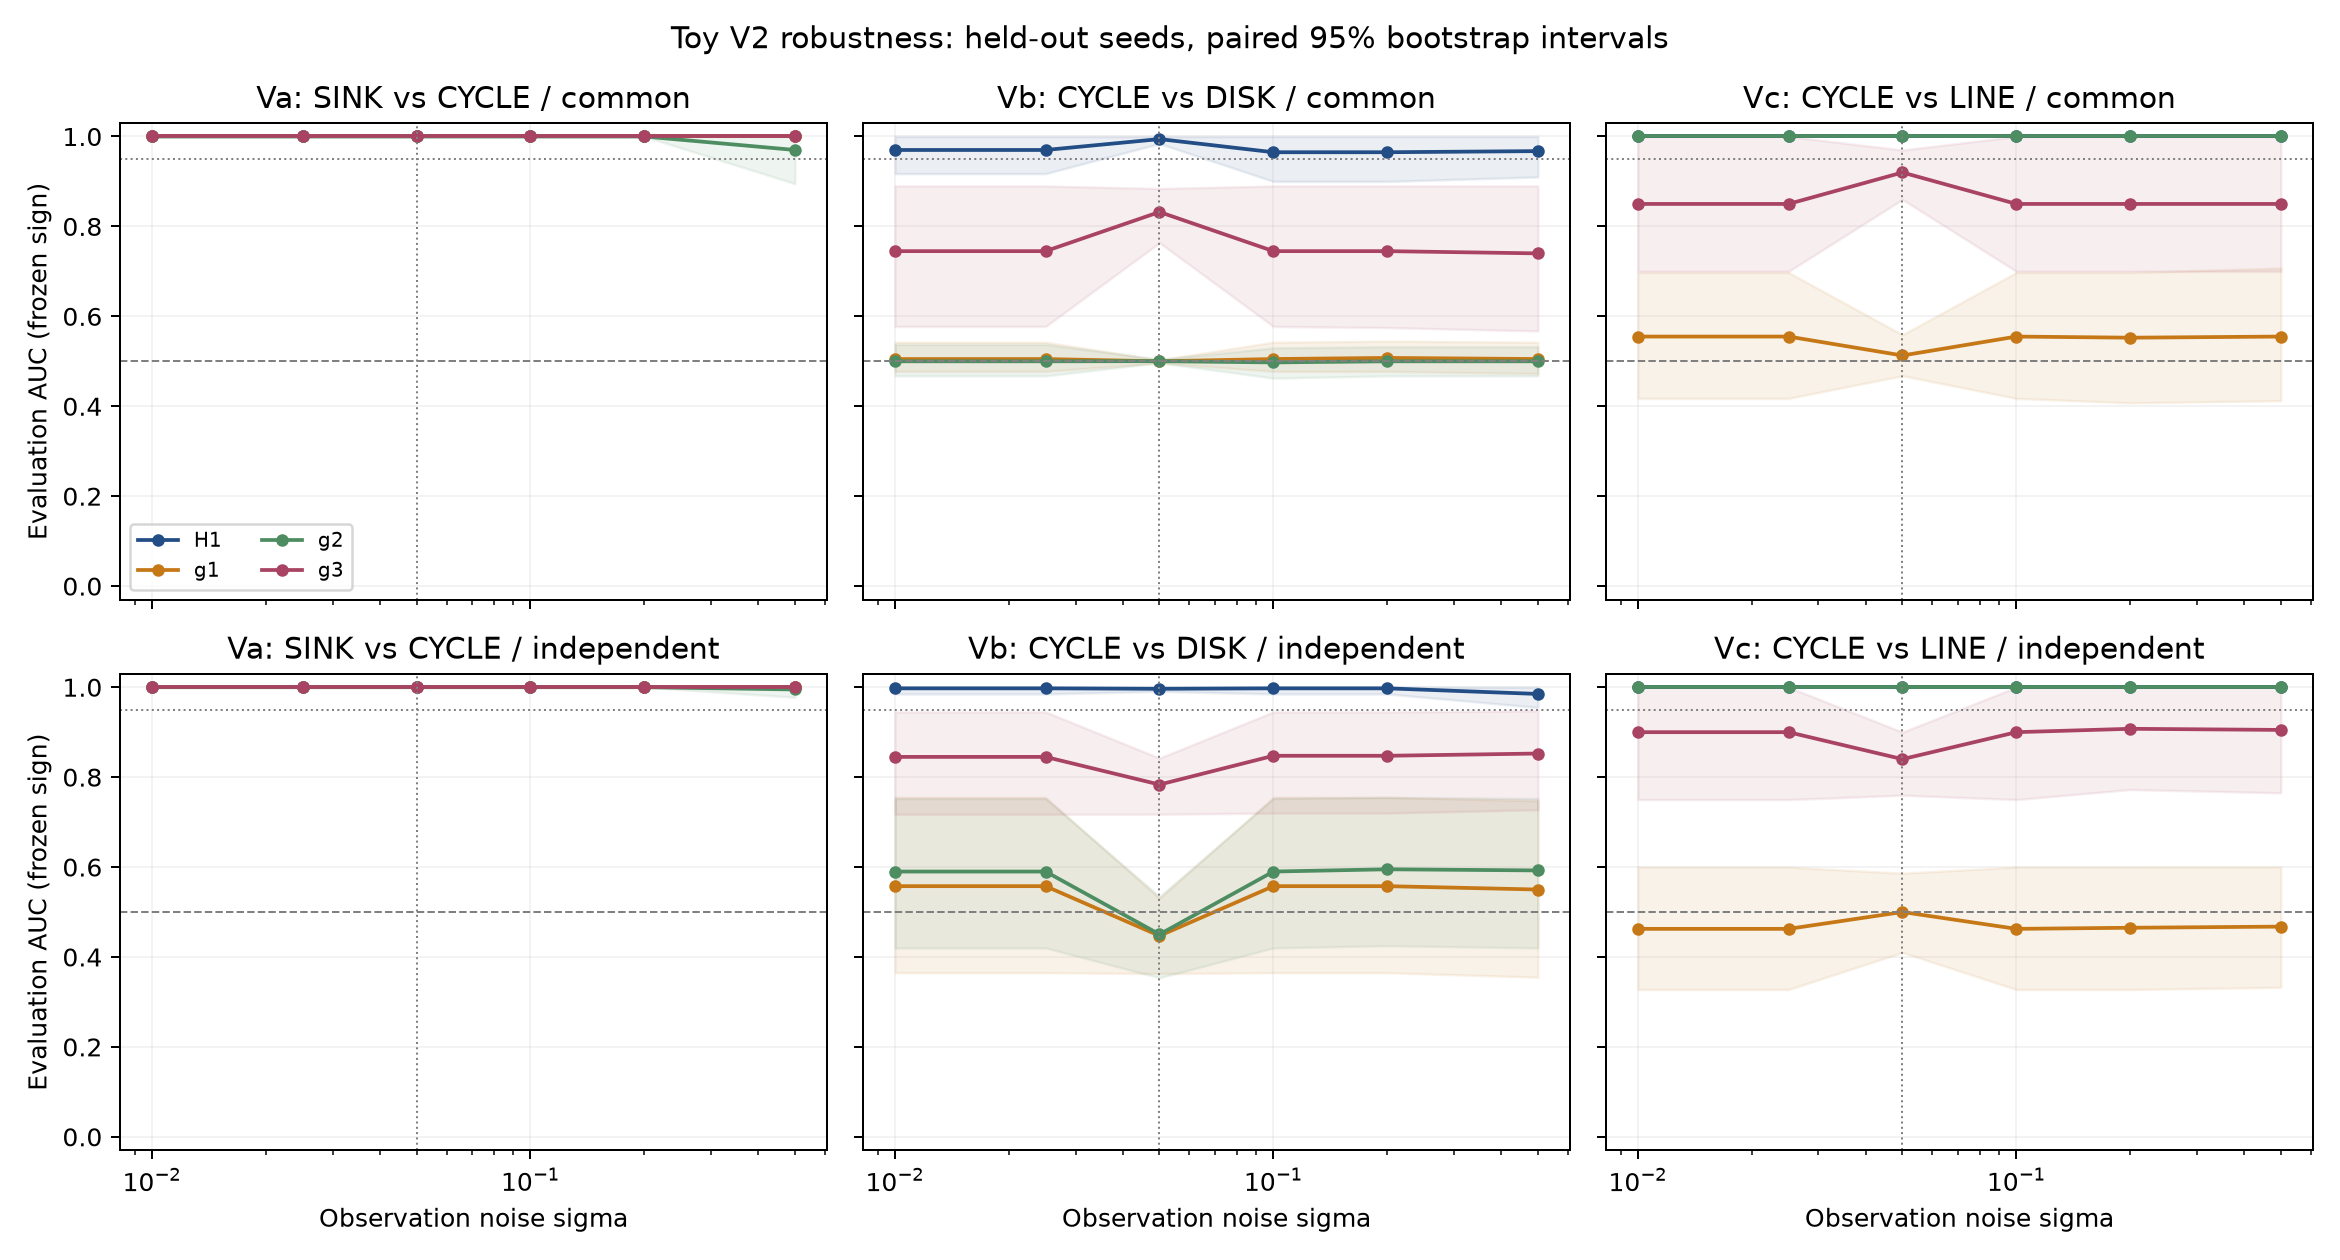
\includegraphics[width=\textwidth]{../experiments/results/toy_v2_robustness/toy_v2_robustness.png}
\caption{Original committed noise sweep, preserved unchanged. The primary noise
point and other points use the different seed sets specified in
Figure~\ref{fig:toy2amendednoise}; all statistics use calibration-frozen signs.}
\label{fig:toy2originalnoise}
\end{figure}

\paragraph{Moment matching, shuffling, reproducibility and limits.}
The maximum GAUSS pre-projection mean and covariance residuals across all seeds
are $3.29\times10^{-15}$ and $2.66\times10^{-15}$; for UNIFORM they are
$3.47\times10^{-16}$ and $2.44\times10^{-15}$. LINE mean and total-variance
residuals are $4.86\times10^{-17}$ and $1.78\times10^{-15}$.
The target pooled AR(1) coefficient is $0.99051344$; realized empirical lag-1
estimates range from $0.95540$ to $0.99667$ before affine matching and from
$0.94809$ to $0.99575$ after it. A fixed affine map commutes with a scalar AR(1)
transition, but a sample-dependent map does not guarantee stationary independent
Gaussian innovations or exact empirical lag-1 matching in the corrected ensemble.

All 800 CYCLE/CYCLE\_SHUF checks pass the absolute $10^{-9}$ tolerance.
The maximum persistence-diagram difference is zero for both $H_0$ and $H_1$;
the largest difference among $g_1$--$g_3$ is $1.51\times10^{-14}$.
Point-cloud $H_1$ measures loop geometry, not temporal return.
Repeated three-seed calculations are bitwise identical; the original
independent-projection seed 1337 still rounds to $0.0326$ and $5.2649$.
The original and supplemental CPU runs take about 211 and 279 seconds,
respectively, including their five-seed benchmarks and reporting.

Per-seed values, frozen thresholds, coefficients, scalers, predictions,
bootstrap intervals, categories, shuffle checks, environment versions and original
output hashes are recorded under
\path{experiments/results/toy_v2_robustness/}, with supplemental outputs in
\texttt{amendment\_1/}. Degenerate bootstrap intervals such as $[1,1]$ describe
the sampled seeds under the fixed construction, not certainty about other
settings. These remain synthetic pipeline checks; none of these results concerns
LLM activations, user identity, or empirical return to an attractor.
\clearpage
\endgroup
